\documentclass{book}
\usepackage[left=2cm, right=2cm, top=2cm, bottom=2cm]{geometry}

\usepackage[spanish]{babel}
\usepackage[utf8]{inputenc}

\usepackage{pdfpages}
\usepackage{hyperref} % Para enlaces y metadatos
\usepackage{fontawesome5}
\usepackage{fancyhdr}
\usepackage{bookmark}

\hypersetup{
    colorlinks=true,
    linkcolor=black,  % Color de los enlaces internos (por ejemplo, dentro de la tabla de contenidos)
    urlcolor=magenta,   % Color de los enlaces a URLs
    %%citecolor=green,
    pdfauthor={Moisés Serrano Samudio},
    pdftitle={Villancicos Populares},
    pdfsubject={partituras},
    pdfkeywords={violín,trío,villancicos}
}

\title{Villancicos Populares}
\author{Moisés Serrano Samudio}
\date{24 octubre 2023}

\begin{document}

\setcounter{page}{1}

\includepdf[pages=-]{../extend/chapter-partituras.pdf}

%\AddToShipoutPictureBG*{ %% Añade imagen al pie de página
%    \AtPageLowerLeft{\put(0,0){\includegraphics[width=\paperwidth,height=2.5cm]{extend/bottom.png}}}%
%}

%%
%% Exportar por individual cada villancico a PDF previamente
%%

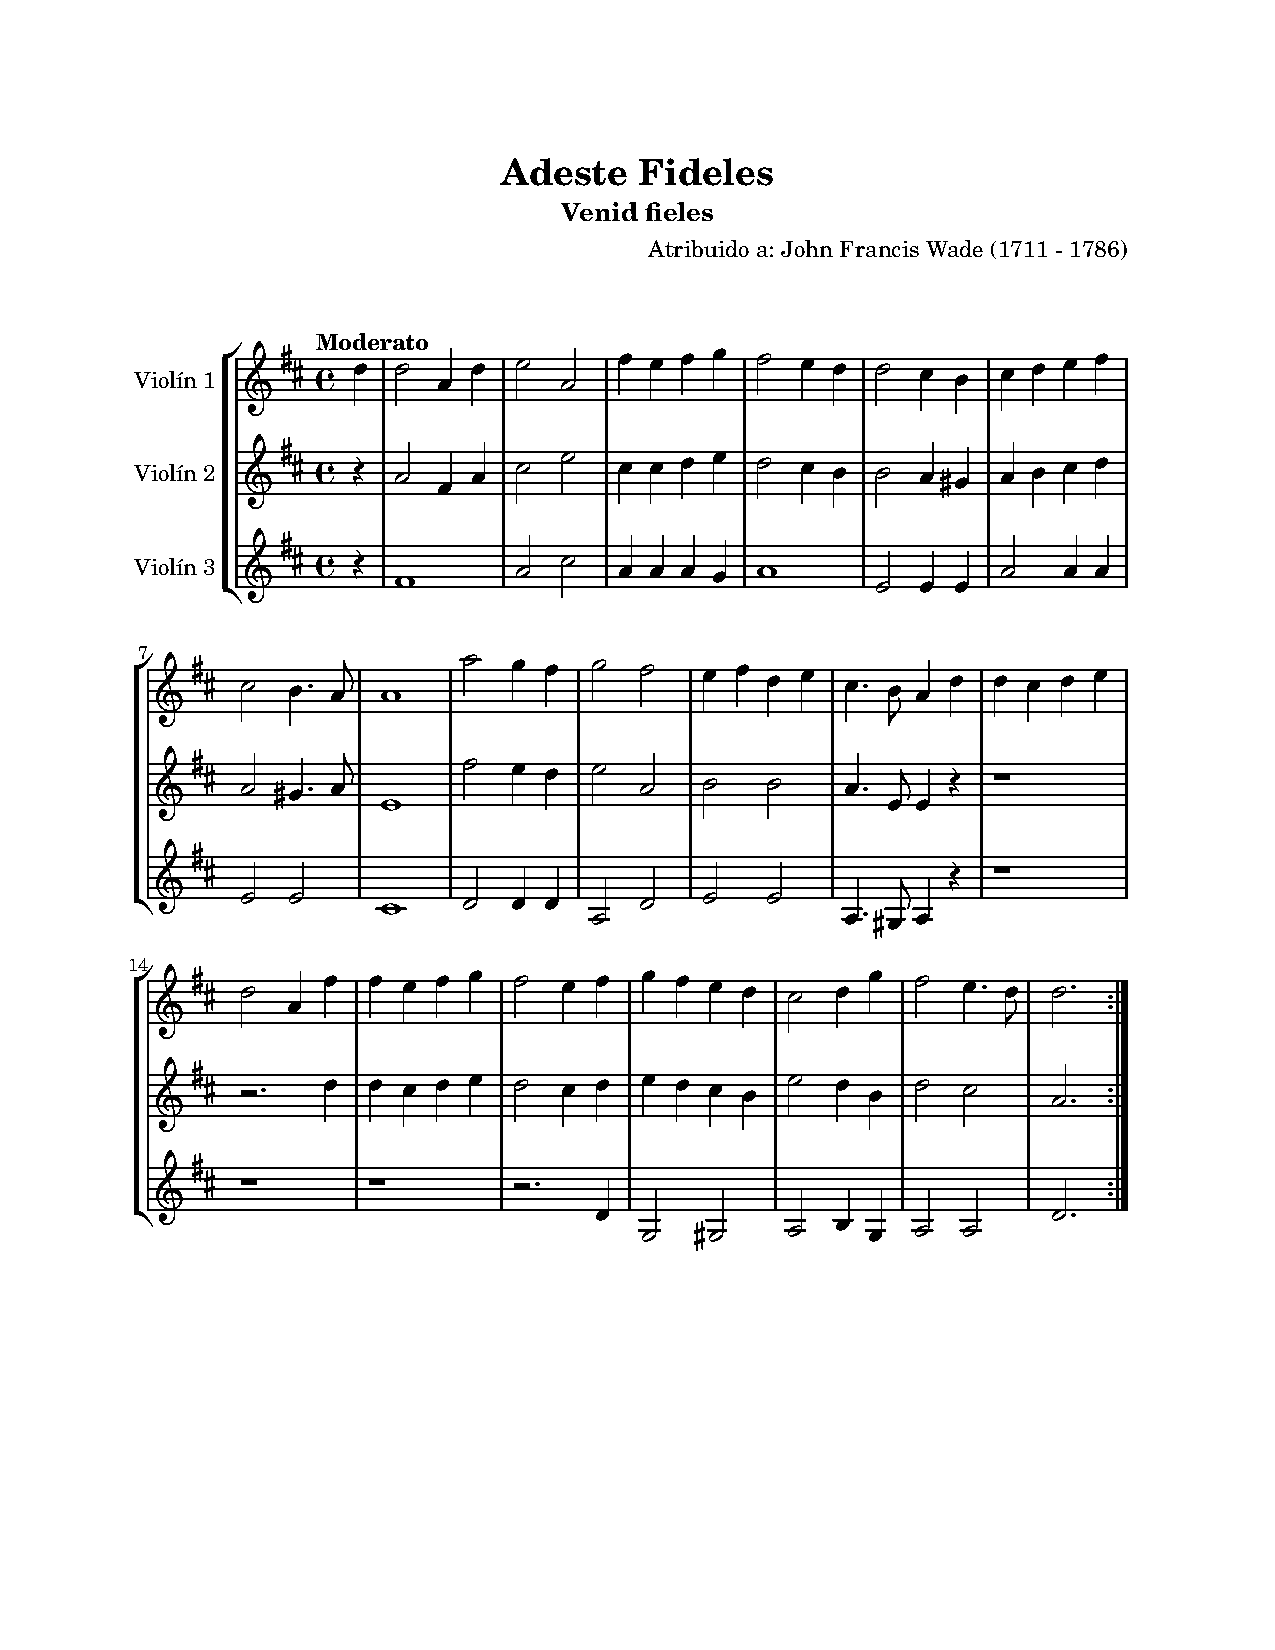
\includepdf[pages=-, pagecommand={\thispagestyle{plain}}]{../adeste-fideles.pdf}

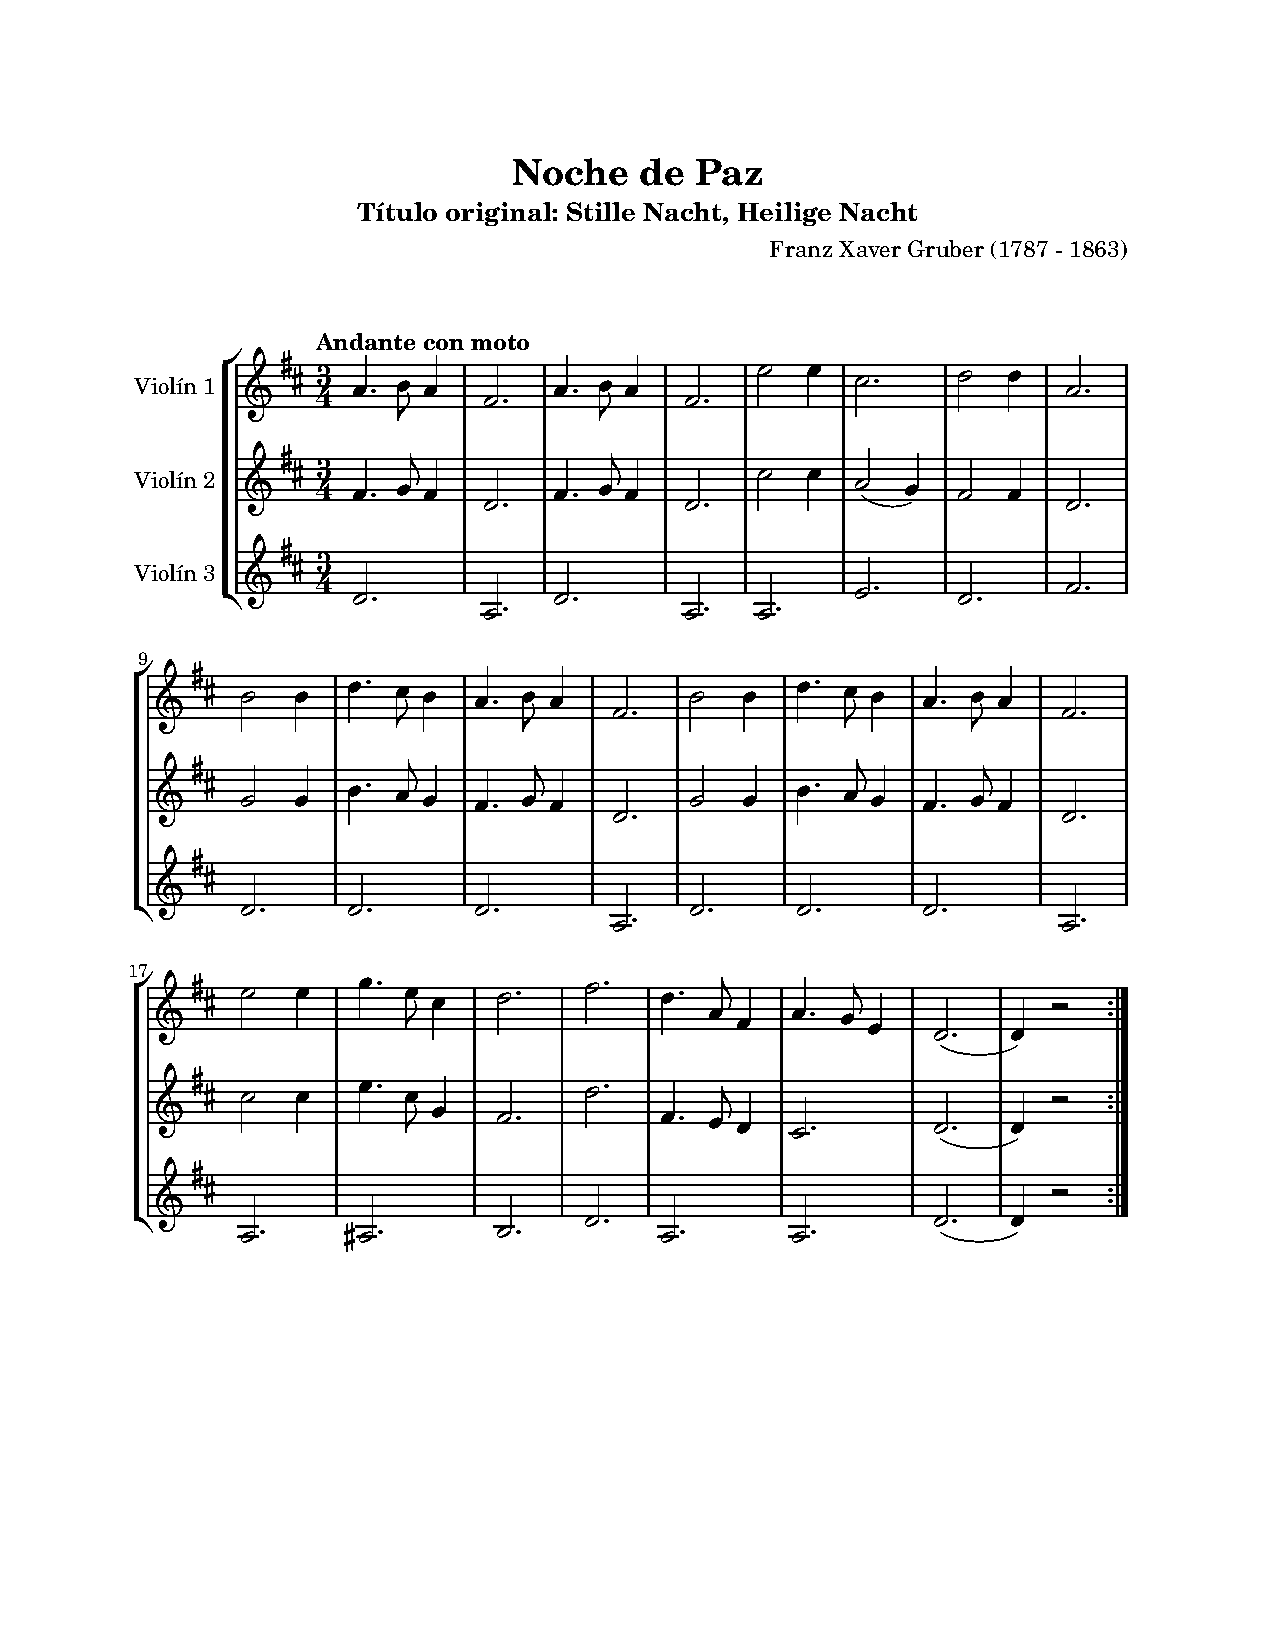
\includepdf[pages=-, pagecommand={\thispagestyle{plain}}]{../noche-de-paz.pdf}

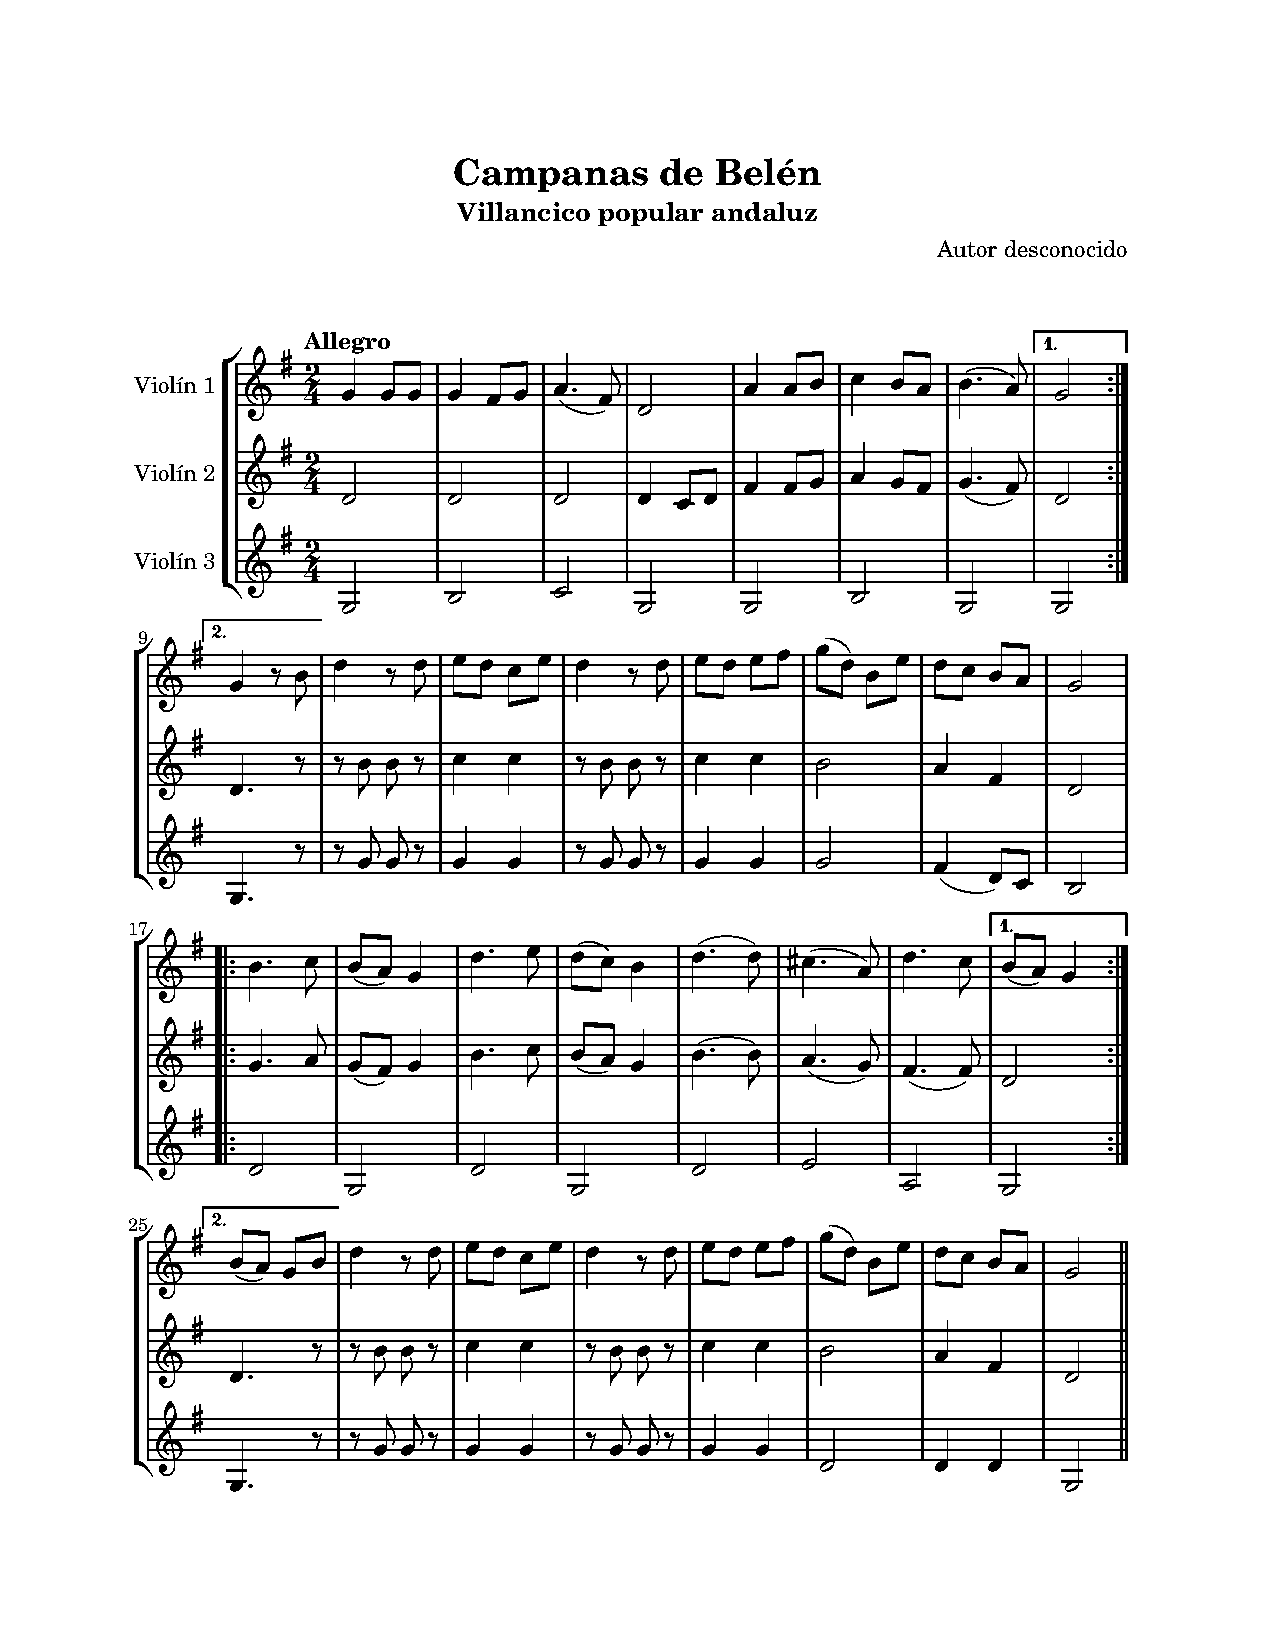
\includepdf[pages=-, pagecommand={\thispagestyle{plain}}]{../campanas-de-belen.pdf}

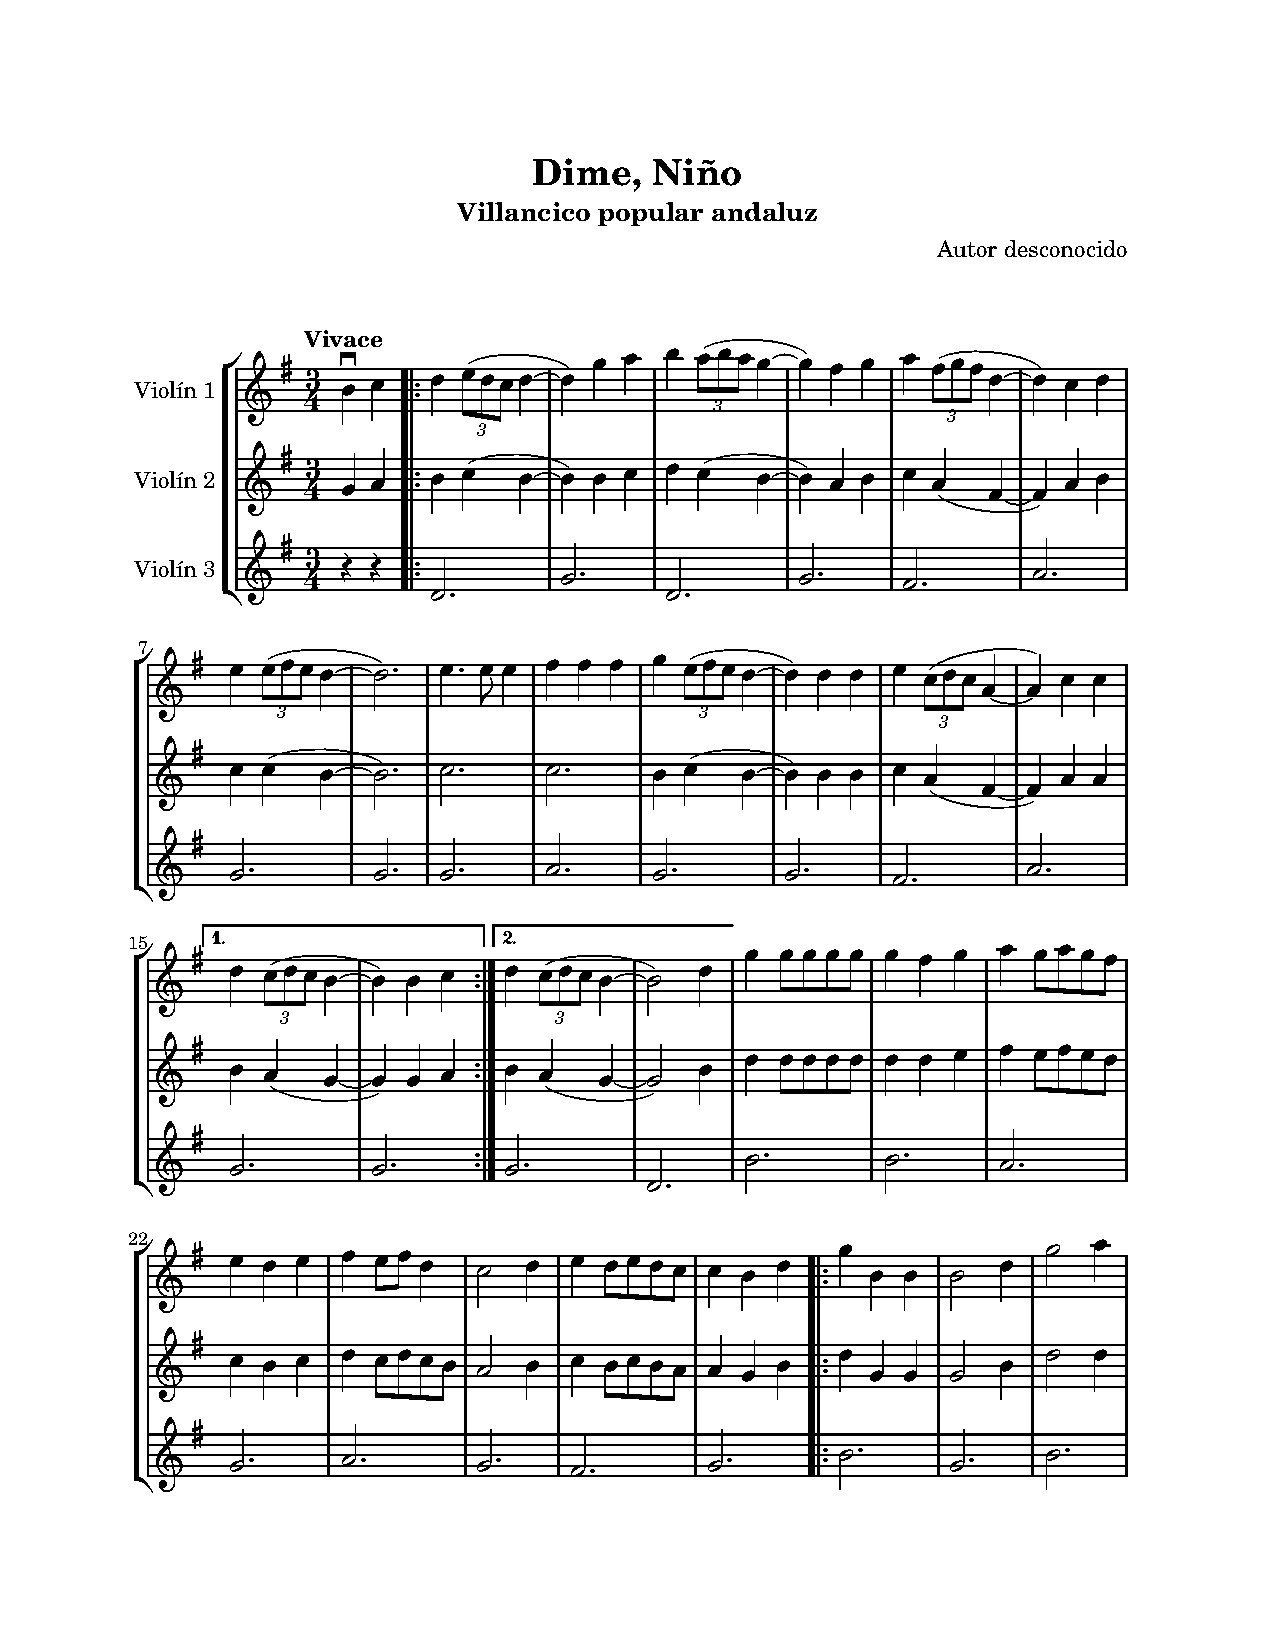
\includepdf[pages=-, pagecommand={\thispagestyle{plain}}]{../dime-niño.pdf}

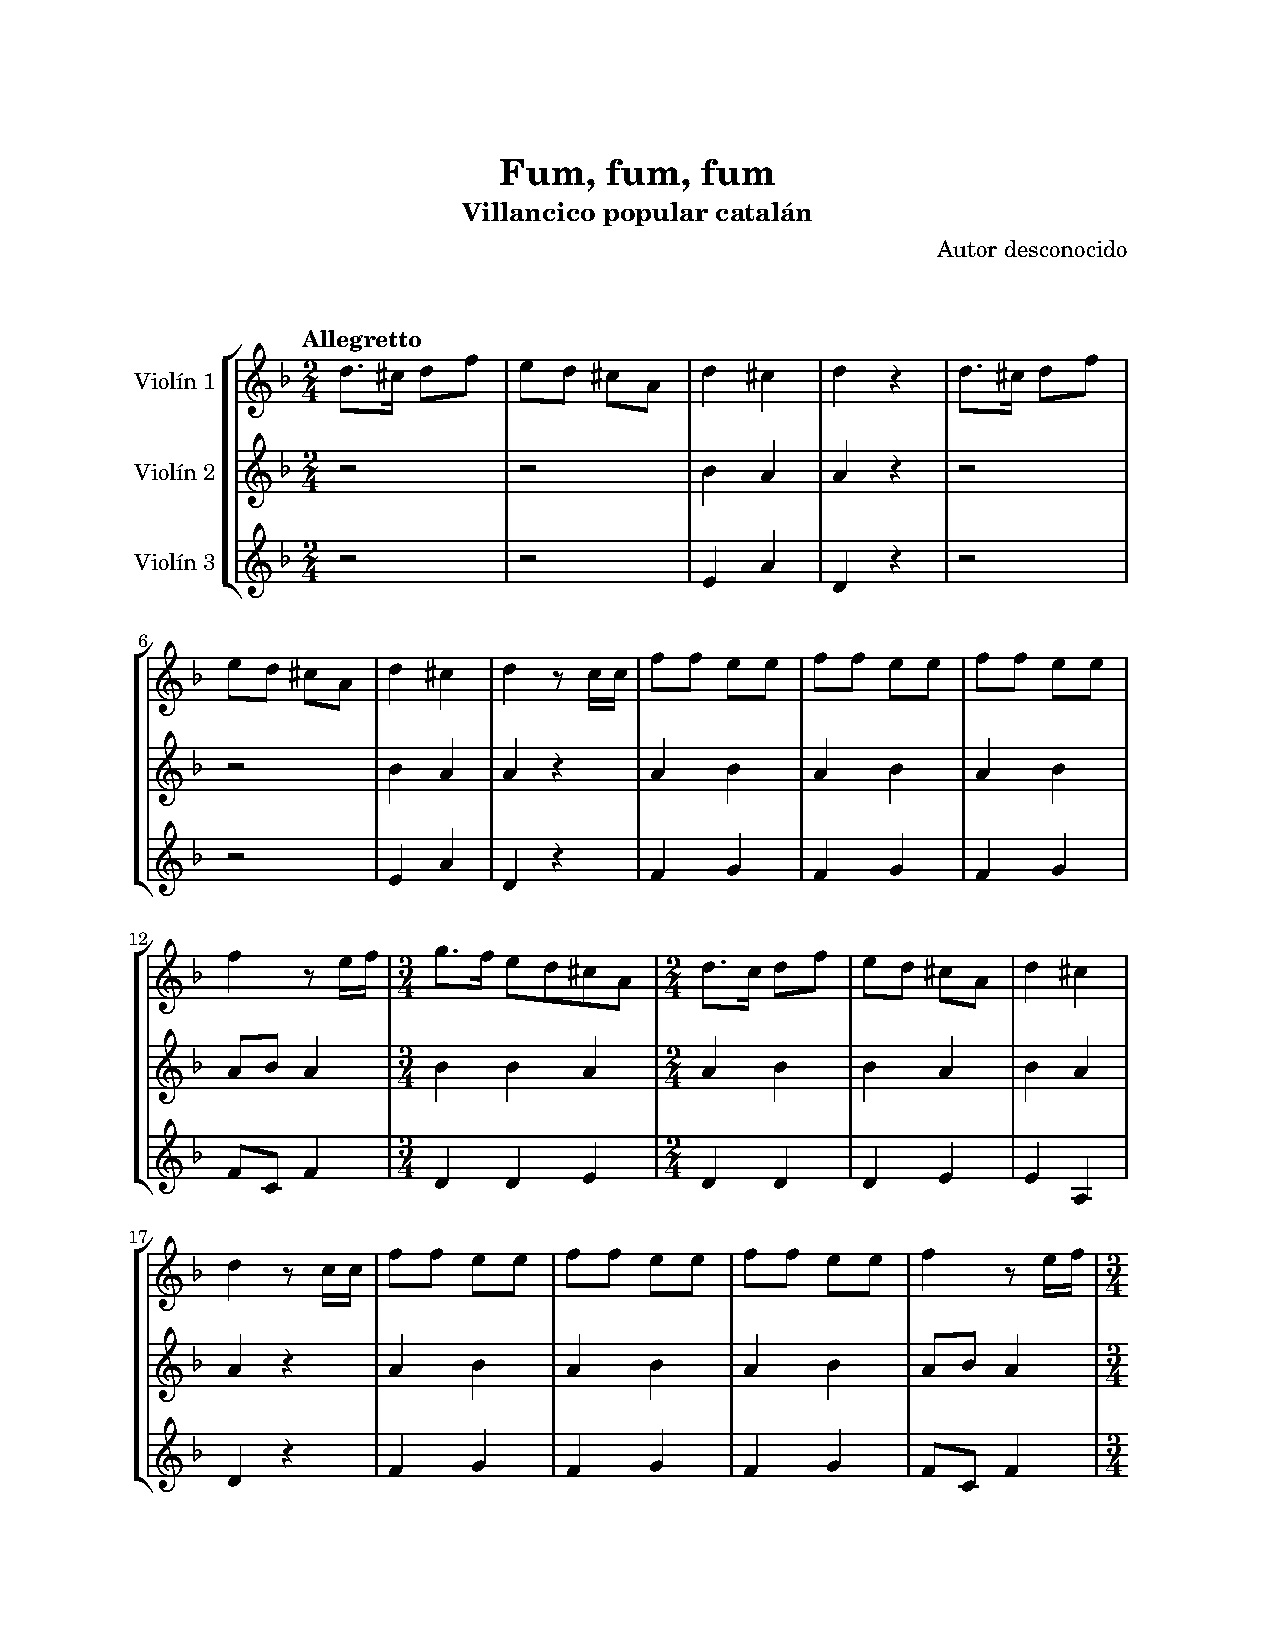
\includepdf[pages=-, pagecommand={\thispagestyle{plain}}]{../fum-fum-fum.pdf}

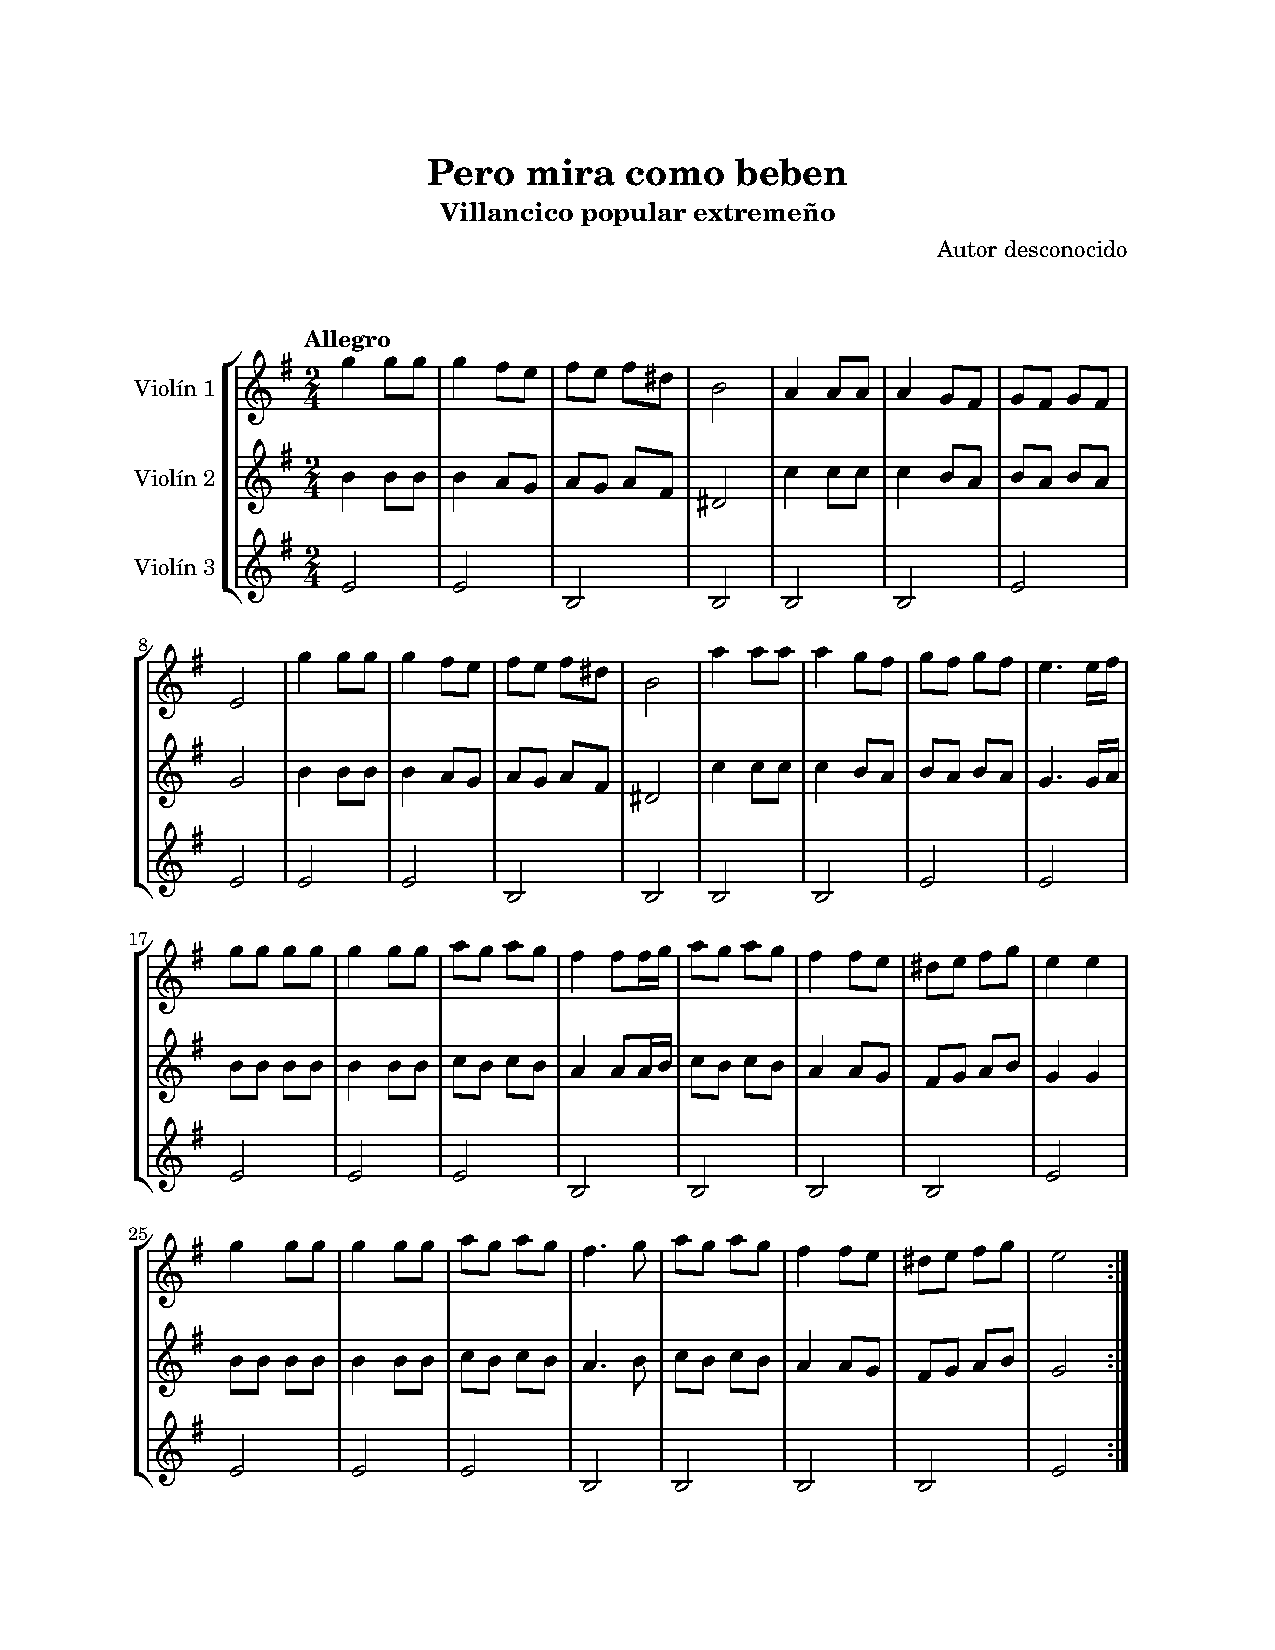
\includepdf[pages=-, pagecommand={\thispagestyle{plain}}]{../pero-mira-como-beben.pdf}

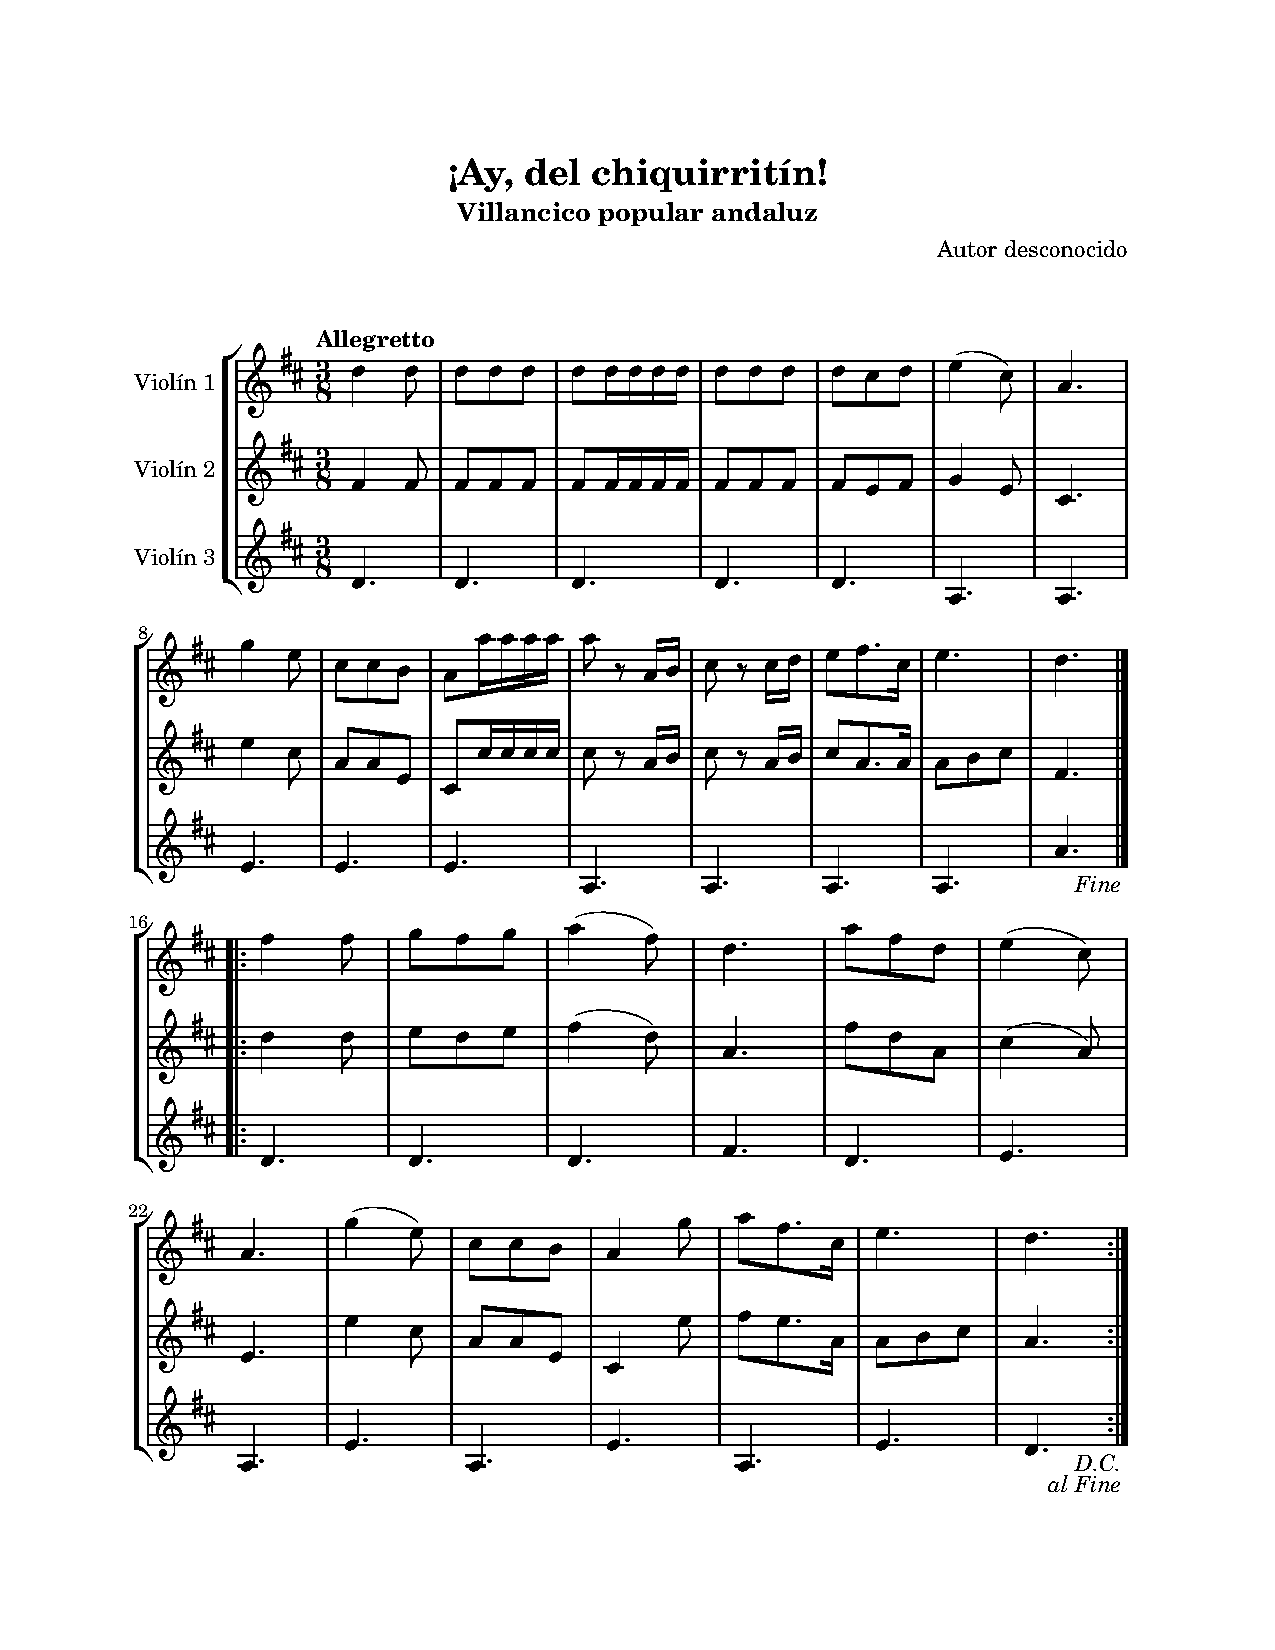
\includepdf[pages=-, pagecommand={\thispagestyle{plain}}]{../ay-del-chiquirritin.pdf}

\includepdf[pages=-, pagecommand={\thispagestyle{plain}}]{../la-marimorena.pdf}

\includepdf[pages=-, pagecommand={\thispagestyle{plain}}]{../alegria-alegria.pdf}

\includepdf[pages=-, pagecommand={\thispagestyle{plain}}]{../rin-rin.pdf}

\includepdf[pages=-, pagecommand={\thispagestyle{plain}}]{../tamborilero.pdf}

\includepdf[pages=-, pagecommand={\thispagestyle{plain}}]{../burrito-sabanero.pdf}

\includepdf[pages=-, pagecommand={\thispagestyle{plain}}]{../feliz-navidad.pdf}

\includepdf[pages=-, pagecommand={\thispagestyle{plain}}]{../nochebuena-pa.pdf}

\includepdf[pages=-, pagecommand={\thispagestyle{plain}}]{../arre-borriquito.pdf}

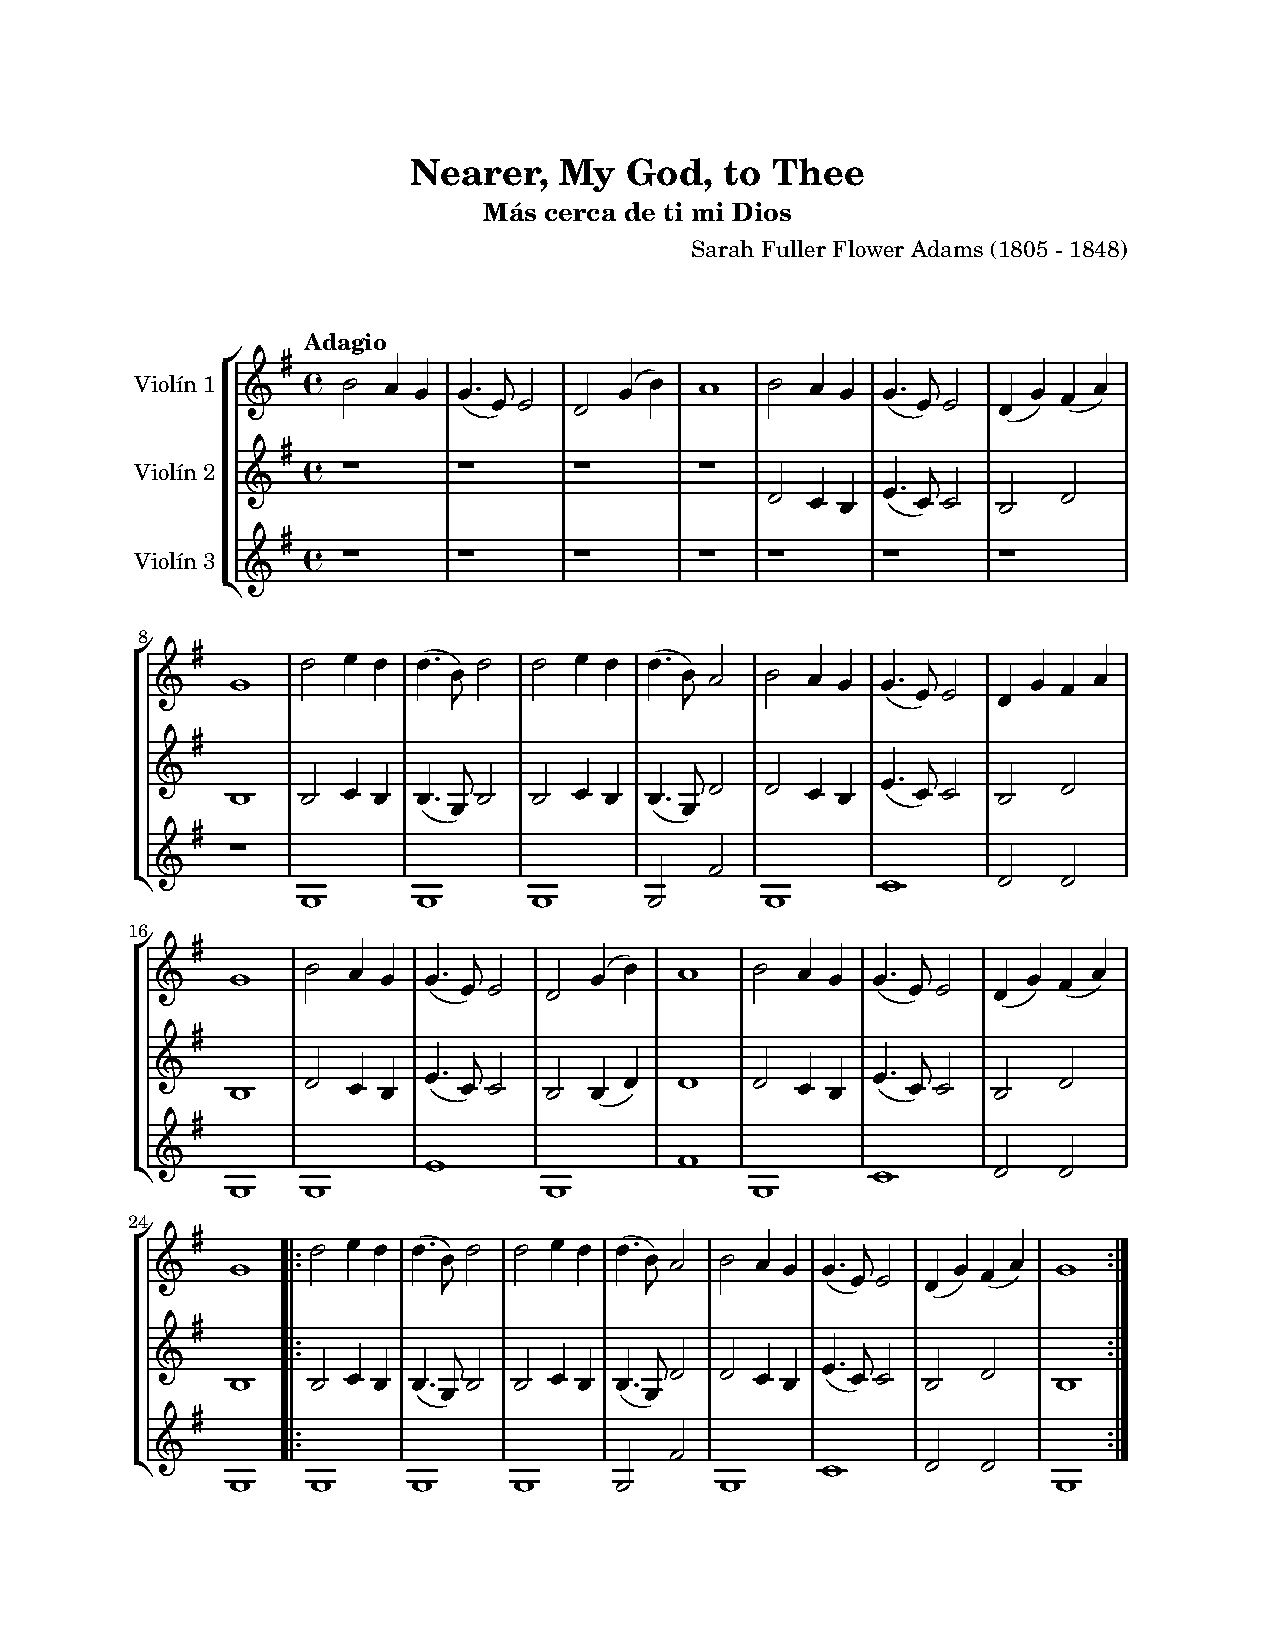
\includepdf[pages=-, pagecommand={\thispagestyle{plain}}]{../nearer-my-god-to-thee.pdf}


\includepdf[pages=-]{../extend/blank.pdf}

\includepdf[pages=-]{../extend/chapter-letras.pdf}

%%
%%  Exportar desde libreoffice en PDF letras-villancicos.odt
%%
%%  rotar la página con pdfjam
%%
%%      $ pdfjam --nup 1x1 --suffix rotado --angle 90 -- letras-villancicos.pdf
%%

\includepdf[pages=-, pagecommand={\thispagestyle{plain}}]{../villancicos-letras-rotado.pdf}

\end{document}